% !TeX TS-program = pdflatex
\documentclass{beamer}

\usepackage{tikz}
\usetikzlibrary{overlay-beamer-styles}
\setbeamertemplate{navigation symbols}{}

\begin{document}

\begin{frame}[plain]%%%%%%%%%%%%%%%%%%%%%%%%%%%%%%%%%%%%%%%%%%%
	\begin{tikzpicture}[remember picture,overlay]
  	\node[at=(current page.center)]{
   		\includegraphics[height=1.05\paperheight,page=\thepage]{ce_why_R_moles_gray}
		};
	\end{tikzpicture}
	\pause[40]
\end{frame}


\begin{frame}[plain]%%%%%%%%%%%%%%%%%%%%%%%%%%%%%%%%%%%%%%%%%%%
	\begin{tikzpicture}[remember picture,overlay]
  	\node[at=(current page.center)]{
   		\includegraphics[height=1.05\paperheight,page=40]{ce_why_R_moles_gray}
		};
	\end{tikzpicture}
	\pause[20]
\end{frame}

\end{document}